\documentclass{ctexart}
\usepackage{EC}
\begin{document}
\section{硅及其化合物}
\subsection{硅单质}
\subsubsection{硅单质的制备}
\paragraph{硅单质的发现}
从硅酸盐矿物中得到硅单质的历史已有两百余年.1808年,Berzelius就尝试用\ce{Fe}和\ce{C}的混合物还原石英\ce{SiO2}以得到\ce{Si}单质,但可惜的是显然他得到的是硅铁.1809年,Davy也从事\ce{Si}单质的制备,但也没有成功.\\
\indent 1811年,Gay Lussac和Thénard用金属钾还原\ce{SiCl4},得到了一种无定形的棕色粉末:
\begin{center}
    \ce{4K + SiCl4 -> 4KCl + Si}
\end{center}
可惜的是,他们并没有认出这种棕色粉末就是硅单质.直到1823年,Berzelius重新用\ce{K}单质还原\ce{K2SiF6}而制得了\ce{Si}单质:
\begin{center}
    \ce{4K + K2SiF6 -> 6KF + Si}
\end{center}
他还对产物进行了细致的清洗,并研究了硅单质的若干性质.因此,一般将\ce{Si}单质的发现人归为Berzelius.
\paragraph{硅单质的工业制备方法I}
\indent 继最早的研究之后,又有发现了许多制备\ce{Si}单质的方法,主要是用碱金属或碱土金属作为还原剂还原含\ce{Si}化合物,或采取放电还原的方式.现在,在工业上制备\ce{Si}单质的方法为将焦炭与过量的\ce{SiO2}共热:
\begin{center}
    \ce{SiO2 + 2C ->T[$\Delta$] Si + 2CO}
\end{center}
显然地,\ce{SiO2}过量可以防止难以分离的\ce{SiC}的生成.这样得到的硅单质纯度大约为$97\sim98\%$.将其熔融后重结晶,再经过酸洗后即得到纯度为$99.7\sim99.8\%$的纯硅.如果需要制得高纯度的半导体硅,首先可以用\ce{HCl}与\ce{Si}单质反应得到\ce{SiHCl3}:
\begin{center}
    \ce{Si + 3HCl ->T[$280\sim320\tc$][\ce{CuCl}] SiHCl3 + H2}
\end{center}
随后将得到的混合物(其中的主要杂质是其它元素的氯化物,例如\ce{AlCl3}等)进行精馏而得到较纯的\ce{SiHCl3},然后在高温下用\ce{H2}还原并采取气相沉积法(CVD)收集\ce{Si}即可得到多晶\ce{Si}单质:
\begin{center}
    \ce{SiHCl3 + H2 ->T[$1100\tc$] Si + 3HCl}
\end{center}
这样制得的硅单质纯度在$\underbrace{99.99999}_{\text{7个9}}\%$到$\underbrace{99.9999999}_{\text{9个9}}\%$左右.通常,我们用$xN$表示硅单质杂质含量少于$10^{-x}$,因此这样制得的多晶硅纯度为$7N$到$9N$.
\paragraph{硅单质的工业制备方法II}
如果想要制备纯度为$11N$及以上的单晶硅,还需要区域熔炼法或提拉法继续提纯.\\
\indent 提拉法又称柴可拉斯基法(Czochralski Process),其过程如下所示.
\chemfig{Czochralski_Process}{0.4}{提拉法的步骤示意图}
提拉法的步骤为:
\begin{enumerate}[label=$\mathit{Step\ \arabic*.}$,topsep=0pt,parsep=0pt,itemsep=0pt,partopsep=0pt,leftmargin=*]
    \item 将高纯度的多晶硅在坩埚(通常是石英坩埚)中熔融.有时需要按照用途掺杂.
    \item 将晶种连接在一根精确定向的棒的末端.
    \item 使棒的末端浸入熔融的硅单质中.
    \item 缓慢向上提拉棒,同时匀速旋转棒.控制旋转速率,提拉速率和温度,即可在相界面上不断结晶出高纯度的,一定半径的\ce{Si}单质棒.
    \item 将棒与\ce{Si}单质截断,即可得到单晶\ce{Si}.通常,这样的\ce{Si}单质可以被直接切割为晶圆(即圆形的单晶\ce{Si}薄片),然后用于芯片等的生产.
\end{enumerate}

\indent 区域熔炼法则是根据相平衡的原理进行提纯的.我们以提纯\ce{Si}为例,其中的杂质的存在将导致凝固点发生变化.
\begin{figure}[H]
    \centering\documentclass{standalone}
\usepackage{PhysicalChemistryNote}
\begin{document}
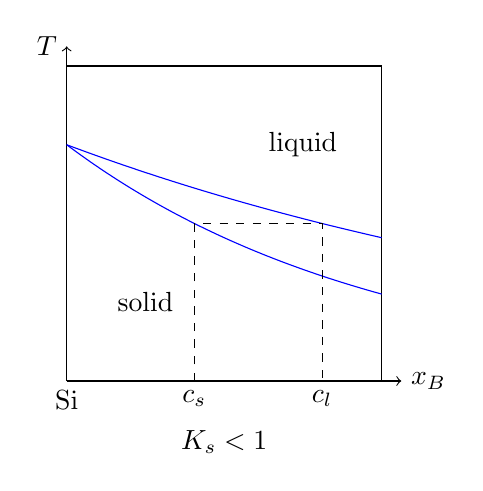
\begin{tikzpicture}
    \draw[->] (0,0) -- (4.25,0) node[right] {$x_B$};
    \draw[->] (0,0) -- (0,4.25) node[left]{$T$};
    \draw[-] (4,0) -- (4,4);
    \draw[-] (0,4) -- (4,4);
    \node[below] at (0,0) {Si};
    \draw[domain=0:4,blue] plot[smooth](\x,{3*e^(-\x/4)});
    \draw[domain=0:4,blue] plot[smooth](\x,{3*e^(-\x/8)});
    \draw[dashed] (1.6218,0)--(1.6218,2)--(3.2437,2)--(3.2437,0);
    \node[below] at (1.6218,0) {$c_{\text s}$};
    \node[below] at (3.2437,0) {$c_{\text l}$};
    \node[below] at (2,-0.5) {$K_s<1$};
    \node at (1,1) {solid};
    \node at (3,3) {liquid};
\end{tikzpicture}
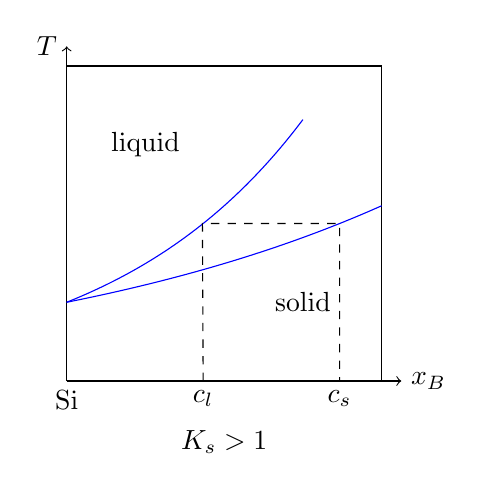
\begin{tikzpicture}
    \draw[->] (0,0) -- (4.25,0) node[right] {$x_B$};
    \draw[->] (0,0) -- (0,4.25) node[left]{$T$};
    \draw[-] (4,0) -- (4,4);
    \draw[-] (0,4) -- (4,4);
    \node[below] at (0,0) {Si};
    \draw[domain=0:3,blue] plot[smooth](\x,{e^(\x/2.5)});
    \draw[domain=0:4,blue] plot[smooth](\x,{e^(\x/5)});
    \draw[dashed] (1.7329,0)--(1.7239,2)--(3.4657,2)--(3.4657,0);
    \node[below] at (1.7329,0) {$c_{\text l}$};
    \node[below] at (3.4657,0) {$c_{\text s}$};
    \node[below] at (2,-0.5) {$K_s>1$};
    \node at (3,1) {solid};
    \node at (1,3) {liquid};
\end{tikzpicture}
\end{document}
    \caption{熔融液体凝固时固相中的杂质含量变化}
\end{figure}
图中纵坐标为温度,横坐标为杂质$B$的含量$x_B$,在固相线和液相线之间为两相共存区.在一定温度下,令杂质在固相和液相中的浓度为$c_{\text s}$和$c_{\text l}$.设\tbf{分凝系数}$K_s$满足
\[K_s=\dfrac{c_{\text s}}{c_{\text l}}\]
\indent 先讨论$K_s<1$的情形.假设熔炼区域从左向右移动,那么在熔融区的左侧正在发生重新凝固.凝固时,固相中杂质的浓度小于液相,因此杂质更多地被分配在液相中,于是随着熔炼区域的右移而右移.这样多次重复后,杂质就被扫到最右侧,而左侧就是纯度较高的物质.\\
\indent 对于$K_s>1$的情形,杂质更多地被分配在重新凝固的左侧,因此右侧是纯度较高的物质.\\
\indent 在\ce{Si}中,所有杂质的$K_s<1$,所以经过区域熔炼后杂质集中在尾部.对于\ce{Ge}而言,\ce{B}和\ce{Si}的$K_s>1$,其余杂质的$K_s<1$,因此纯的\ce{Ge}集中在中部,应弃去头尾.\\
\indent 区域熔炼的效率一方面取决于$K_s$的大小,一方面取决于提纯前物质的纯度.$K_s$越远离$1$,提纯前的物质越纯,区域熔炼的效率越高.于是进行区域熔炼法之前一般要用其他方法,例如化学法进行提纯.区域熔炼法也可以用于有机物的提纯和高分子化合物的分类,并且能达到很好的效果,因为区域熔炼法可以重复多次.
\subsubsection{硅单质的结构}
一般的单晶硅与金刚石的结构相似,以立方金刚石结构为主.
\chemfig{Si}{0.1}{单晶硅的晶体结构}
由于单晶硅的表面性质与表面的方向密切相关,因此这里简单地介绍一些有关晶面的知识.
\paragraph{晶面指数,晶面间距与晶棱}
晶面是晶体中由周期性排列的原子所形成的几何平面,它反映了晶体内部结构的对称性与规律性,同时对晶体的物理和化学性质有重要影响.例如解理面往往就是特定的晶面.\\
\indent 为了精确描述晶面取向,人们引入了密勒指数(Miller indices).密勒指数用一组三个整数 
$(hkl)$表示某一晶面,其求法如下:
\begin{enumerate}[label=$\mathit{Step\ \arabic*.}$,topsep=0pt,parsep=0pt,itemsep=0pt,partopsep=0pt,leftmargin=*]
    \item 假设欲求指标的晶面$S$与晶格的单位向量$\mbf a,\mbf b,\mbf c$方向上的截距分别为$pa,qb,rc$,其中$a,b,c$为晶胞参数,$p,q,r$为正整数.
    \item 当晶面$S$与某一单位向量平行时,截距即为$\infty$.为了避免$\infty$的出现,因此将$p,q,r$分别取倒数得到$\dfrac1p:\dfrac1q:\dfrac1r$,截距为$\infty$时倒数就为$0$.
    \item 将$\dfrac1p,\dfrac1q,\dfrac1r$化为最简整数比$h:k:l$,那么这一晶面的Miller指数即为$(hkl)$.如果需要指代一组空间上等价的晶面,则可以改为用花括号表示,即$\{hkl\}$.
\end{enumerate}
下面给出了立方晶胞的常见的晶面.
\begin{figure}[H]
    \centering
    \subfigure[$(100)$]{
        \begin{minipage}[b]{.3\linewidth}
            \centering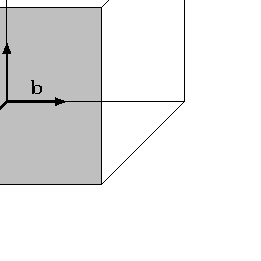
\includegraphics[scale=0.75]{picture/100.tex}
        \end{minipage}
    }
    \subfigure[$(010)$]{
        \begin{minipage}[b]{.3\linewidth}
            \centering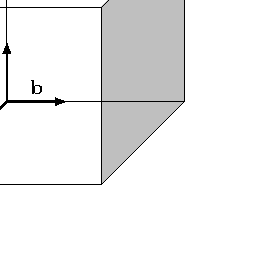
\includegraphics[scale=0.75]{picture/010.tex}
        \end{minipage}
    }
    \subfigure[$(001)$]{
        \begin{minipage}[b]{.3\linewidth}
            \centering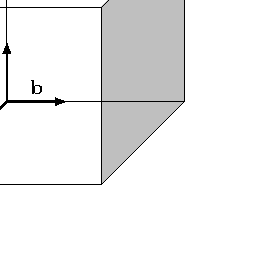
\includegraphics[scale=0.75]{picture/010.tex}
        \end{minipage}
    }
    \subfigure[$(110)$]{
        \begin{minipage}[b]{.3\linewidth}
            \centering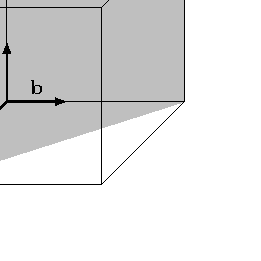
\includegraphics[scale=0.75]{picture/110.tex}
        \end{minipage}
    }
    \subfigure[$(102)$]{
        \begin{minipage}[b]{.3\linewidth}
            \centering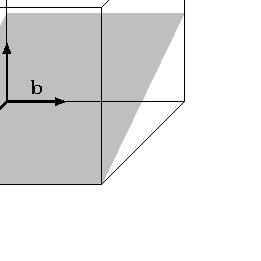
\includegraphics[scale=0.75]{picture/102.tex}
        \end{minipage}
    }
    \subfigure[$(111)$]{
        \begin{minipage}[b]{.3\linewidth}
            \centering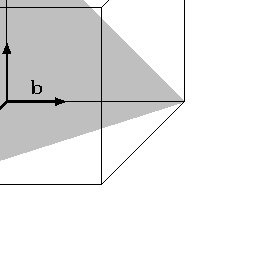
\includegraphics[scale=0.75]{picture/111.tex}
        \end{minipage}
    }
    \caption{立方晶胞中的常见晶面示意图}
\end{figure}
有关晶面的另一个重要参数是晶面间距.在立方晶胞中,Miller指数为$\{hjl\}$的一组晶面的相邻间距为
\[\dfrac{a}{\sqrt{h^2+k^2+l^2}}\]
这可以通过简单的立体几何知识算得,这里就不加以详细推导了.\\
\indent 通常容易形成的晶面(例如晶体自然结晶形成的规则几何外形的面或解理时形成的面)都是Miller指数较小的面.Miller指数小一般意味着晶面间距更大,晶面上的原子数目更多,相互作用更强,表面能也就更低.\\
\indent 既然有晶面以描述晶体中的面,那么很自然地也能想到\tbf{晶棱}(或称\tbf{晶向})以描述晶体中的线或方向.我们仿照空间向量的分解方法,将描述某一特定方向的向量$\mbf l$按照如下方式分解:
\[\mbf l=u_0\mbf a+v_0\mbf b+w_0\mbf c\]
然后将$u_0:v_0:w_0$化为最简整数比$u:v:w$,那么这一向量$\mbf l$所指代的方向的\tbf{晶棱指数}(或称\tbf{晶向指数})就记作$[uvw]$.\\
\indent 我们接下来给出一个有趣而简单的事实:立方晶系中晶面指数为$(hkl)$的晶面的法向量$\mbf u$的晶向指数也为$[hkl]$.
\begin{proof}
    这一事实等价于:与直角坐标系中三个坐标轴的截距分别为$\dfrac1h,\dfrac1k,\dfrac1l$的平面$S$的法向量为$\mbf u=(h,k,l)$.\\
    为此,我们取平面上的两个向量$\mbf i=\left(\dfrac1h,0,-\dfrac1l\right)$和$\mbf j=\left(\dfrac1h,-\dfrac1k,0\right)$(对于不存在截距的情况作特殊讨论).不难得出:
    \[\mbf i\cdot\mbf u=\dfrac1h\cdot h+0\cdot k+\left(-\dfrac1l\right)\cdot l=0\]
    \[\mbf j\cdot\mbf u=\dfrac1h\cdot h+\left(-\dfrac1k\right)\cdot k+0\cdot l=0\]
    于是$\mbf i$和$\mbf j$均与$\mbf u$垂直.这意味着$S$平面上有两条相交的直线与$\mbf u$垂直,因此$S\bot\mbf u$.\\
    这一结论不仅在晶体学中有应用,在高中的立体几何学中也有重要而广泛地应用.利用这一结论,我们可以迅速地写出平面的法向量,从而避免繁琐而容易出错的联立计算.
\end{proof}
\paragraph{单晶硅的晶面}
单晶硅的应用中所使用的晶面主要为$(100),(110),(111)$等.这三种晶面的原子排列方式如下所示:
\begin{figure}[H]
    \centering
    \subfigure[$(100)$]{
        \begin{minipage}[b]{.3\linewidth}
            \centering\includegraphics[scale=0.8]{picture/Si001.eps}
        \end{minipage}
    }
    \subfigure[$(110)$]{
        \begin{minipage}[b]{.3\linewidth}
            \centering\includegraphics[scale=0.8]{picture/Si110.eps}
        \end{minipage}
    }
    \subfigure[$(111)$]{
        \begin{minipage}[b]{.3\linewidth}
            \centering\includegraphics[scale=0.8]{picture/Si111.eps}
        \end{minipage}
    }
    \caption{单晶硅的三种主要晶面}
\end{figure}
为了比较这三种晶面的性质,我们先分别计算各晶面的\tbf{原子面密度}(即单位面积晶面上的原子数目),\tbf{共价键面密度}(即单位面积相邻晶面内的共价键数目)以及晶面法向量方向的\tbf{原子线密度}(即单位长度内的原子数目).
\begin{enumerate}[label=\tbf{\arabic*.},topsep=0pt,parsep=0pt,itemsep=0pt,partopsep=0pt]
    \item $(100)$晶面.\\
        我们不难看出,在一个晶胞内有$4$个与$(100)$晶面等价的晶面.一个晶面上的原子面密度为
        \[\rho_{(100)}=\dfrac{2}{a^2}\]
        对于$(100)$晶面,考虑其上边长为$a$的正方形,观察晶胞可得它和相邻的晶面(过$\left(\dfrac34,0,0\right)$且平行于$yz$平面)之间一共成键的数目为$4$.事实上这与每个原子在这两个面间成键的数目为2等价,因此共价键面密度为
        \[P_{(100)}=\dfrac{4}{a^2}\]
        (100)晶面的法向量即为晶胞的$x$轴向量.在长度为$a$上的原子的数目为1,于是原子线密度为
        \[D_{[100]}=\dfrac{1}{a}\]
    \item $(110)$晶面.\\
        同样不难得到原子面密度为
        \[\rho_{(110)}=\dfrac{4}{\sqrt2a^2}=\dfrac{2\sqrt2}{a^2}\]
        观察可以得到相邻的$(110)$面之间每个原子只连出一根共价键,因此共价键面密度为
        \[P_{(100)}=\dfrac{2\sqrt2}{a^2}\]
        $[110]$方向即为晶胞的面对角线,考察此线上的原子数目即可得出原子线密度
        \[D_{[110]}=\dfrac{2}{\sqrt2a}=\dfrac{\sqrt2}{a}\]
    \item $(110)$晶面.\\
        同样不难得到原子面密度为
        \[\rho_{(111)}=\dfrac{2}{\dfrac{\sqrt3}{4}\left(\sqrt2a\right)^2}=\dfrac{4\sqrt3}{3a^2}\]
        对于金刚石型的晶体,其沿对角线的堆积方式为$AaBbCc$.不难看出,每个字母都代表一种$(111)$晶面,因此$(111)$晶面所相邻的$(111)$晶面有两种类型.一种是$A-a$类型的,这两个晶面之间每个原子成1根键;另一种是$a-B$类型的,这两个晶面之间每个原子成三根键.因此共价键面密度分别为
        \[P_{(111),1}=\dfrac{4\sqrt3}{3a^2}\ \ \ \ \ P_{(111),2}=3\cdot\dfrac{4\sqrt3}{3a^2}=\dfrac{4\sqrt3}{a^2}\]
        $[111]$方向即为晶胞的体对角线,考察此线上的原子数目即可得出原子线密度
        \[D_{[111]}=\dfrac{2}{\sqrt3a}=\dfrac{2\sqrt3}{3a}\]
\end{enumerate}
我们把上述结果整理成一张表格以供参考:
\begin{table}[H]\centering
    \renewcommand\arraystretch{1.6}
    \begin{tabular}{|c|c|c|c|}\hline
        晶面    &原子面密度$\rho$   &共价键面密度$P$    &原子线密度$D$ \\\hline
        $(100)$ &$\dfrac{2}{a^2}$   &$\dfrac{4}{a^2}$   &$\dfrac{1}{a}$\\\hline
        $(110)$ &$\dfrac{2\sqrt2}{a^2}$   &$\dfrac{2\sqrt2}{a^2}$   &$\dfrac{\sqrt2}{a}$\\\hline
        $(111),Aa$ &$\dfrac{4\sqrt3}{3a^2}$   &$\dfrac{4\sqrt3}{3a^2}$   &$\dfrac{2\sqrt3}{3a}$\\\hline
        $(111),aB$ &$\dfrac{4\sqrt3}{3a^2}$   &$\dfrac{4\sqrt3}{a^2}$   &$\dfrac{2\sqrt3}{3a}$\\\hline
    \end{tabular}
\end{table}
可以看出$(111)$晶面的$Aa$面之间的共价键面密度最小,这意味着沿此面解理时需要断裂的共价键最少.因此,单晶硅和金刚石的解理面为$(111)$面.这也造成金刚石一般结晶成八面体结构.\\
\indent 而发生化学腐蚀时,需要按层破坏所有共价键,此时$(111)$晶面的$aB$面之间极高的共价键面密度会阻止沿此方向的腐蚀.然而,由于腐蚀机理的不同,单晶硅和金刚石的腐蚀最快的晶面却不相同.\\
\indent 对于单晶硅而言,发生化学腐蚀的速率为
\[(100)>(110)>(111)\]
这与原子线密度$D$的顺序一致,$D$越小则腐蚀速率越快.然而,发生氧化反应的速率为
\[(111)>(110)>(100)\]
这与原子面密度$\rho$的顺序一致,$\rho$越大则氧化速率越快.然而,对于金刚石而言,发生腐蚀的速率却为
\[(110)>(100)>(111)\]
尚不清楚上述速率所用的数据是否准确,也尚不清楚如何科学地解释这些现象的原因.这有待查证.
\subsubsection{硅单质的化学性质}
除了在高温下,晶状的硅单质一般是动力学上惰性的,这可能是因为在硅的表面形成\ce{SiO2}保护层所致.加热到大约$1000\tc$时,\ce{Si}即能和\ce{O2}发生反应,迅速地生成透明的石英:
\begin{center}
    \ce{Si + O2 ->T[$950\sim1160\tc$] SiO2}
\end{center}
而加热至大约$1400\tc$时,\ce{N2}也与\ce{Si}发生反应生成\ce{Si3N4}:
\begin{center}
    \ce{3Si + 2N2 ->T[$1500\tc$] Si3N4}
\end{center}

\indent \ce{Si}单质对一般的酸呈现惰性.强氧化性的酸也会使其形成\ce{SiO2}保护层,而不能完全腐蚀\ce{Si}.在常见的酸中只有\ce{HF}能对\ce{Si}单质进行有效的腐蚀:
\begin{center}
    \ce{Si + 6HF -> 2H2 + H2SiF6}
\end{center}

\indent \ce{Si}表面的保护层对卤素也不大起作用.\ce{F2}在室温下就与\ce{Si}单质发生剧烈的反应,\ce{Cl2}与\ce{Si}单质的反应则需要加热到$300\tc$,而\ce{Br2}或\ce{I2}则需要加热到$500\tc$.\\
\indent 相比固态\ce{Si},液态的\ce{Si}单质则要活泼得多.它与大部分金属和非金属形成硅化物,并且能还原大多数氧化物形成稳定的\ce{SiO2}.这意味着用到液态硅的反应需要特意选择容器,例如\ce{ZrO2}或IVB到VIB族过渡金属的硼化物.
\subsection{硅化物}
\subsubsection{碳化硅\ce{SiC}}
尽管前人进行了一些尝试,但\ce{SiC}的首次合成和确认是在1891年由E. G. Acheson完成的.现在的工业合成方法主要是基于他的工作改进而成的:
\begin{center}
    \ce{SiO2 + 3C ->T[$2000\sim2500\tc$] SiC + 2CO}
\end{center}
\paragraph{\ce{SiC}的合成}
与硅单质的制备不同,为了主要得到\ce{SiC},应当加入稍过量的焦炭.这一反应主要的到$\alpha-\ce{SiC}$,通常是黑色,墨绿色或紫红色的虹彩光泽的晶体.深色主要是各种杂质,例如\ce{Fe}等所致,而虹彩光泽则是由于表面形成的\ce{SiO2}薄膜.
\paragraph{\ce{SiC}的结构}
尽管\ce{SiC}的分子式非常简单,并且看来似乎应当与具有与单晶硅或金刚石一样的结构,但由于原子的不同以及层排列的不同而具有数十种已知的晶型.这些晶型都以金刚石型结构为基础.\\
\indent 最常见的晶型为$\alpha-\ce{SiC}$,大部分正常情况下制备得到的\ce{SiC}是$\alpha$晶型的,它与立方金刚石的结构一致,但一半的\ce{C}被替换为\ce{Si}原子,两者交替排列.此外,另一种简单的晶型为$\beta-\ce{SiC}$,它的结构则与六方金刚石一致.两者的晶体结构如下所示.
\bichemfig{alpha-SiC}{0.1}{$\alpha-\ce{SiC}$的晶体结构}{beta-SiC}{0.1}{$\beta-\ce{SiC}$的晶体结构}{两种简单\ce{SiC}的结构}
除此之外,还有两种主要的碳化硅,即$4\ce{H}-\ce{SiC}$和$6\ce{H}-\ce{SiC}$.它们的晶体结构如下所示.
\bichemfig{4H-SiC}{0.1}{$4\ce{H}-\ce{SiC}$的晶体结构}{6H-SiC}{0.1}{$6\ce{H}-\ce{SiC}$的晶体结构}{另外两种比较常见的\ce{SiC}的结构}
不难看出,$4H-\ce{SiC}$的堆积形式为$AaBbAaCc$,而$6H-\ce{SiC}$的堆积形式为$AaBbCcAaCcBb$.除此之外,还有更加复杂的堆积方式,例如$15R-\ce{SiC}$的堆积方式(省略四面体空隙的原子层)为$ABCACBCABACABCB$.这实际上可以抽象为$ACBAC,BCABA,CABCB$的三部分,因此$15R-\ce{SiC}$属于$R$心六方点阵.
\paragraph{\ce{SiC}的性质与反应}
\ce{SiC}的热稳定性比硅的任何其它二元化合物都好,它在温度高达约$2700\tc$时,才分解出\ce{Si}.\ce{SiC}不受大多数酸的水溶液的侵蚀(甚至\ce{HF}也不能侵蚀\ce{SiC}),但\ce{H3PO4}能与\ce{SiC}反应\footnote{不少元素化学书中都给出了类似的结论,但没有给出反应的方程式.笔者猜想也许是磷酸和表面的\ce{SiO2}发生反应.}.在空气中加热至$1000\tc$以上时才开始被氧化.这是由于表层\ce{SiO2}起着保护作用.如果用熔融的氢氧化物或碳酸盐将\ce{SiO2}除去,则很容易迅速地发生氧化反应:
\begin{center}
    \ce{SiC + 4NaOH + 2O2 -> Na2SiO3 + Na2CO3 + 2H2O}
\end{center}
相比\ce{Si},\ce{SiC}更容易与卤素单质反应.\ce{Cl2}在$100\tc$时即可与\ce{SiC}发生剧烈反应得到\ce{SiCl4}和\ce{C}单质.\\
\indent 人们对\ce{SiC}之所以感兴趣主要是由于它是一种极好的磨料.这种磨料不仅好在其固有硬度(Mohs硬度为$9.5$,介于刚玉和金刚石之间),而且还在其具有锋利的边缘.$\alpha-\ce{SiC}$还可作耐火材料,它具有很高的强度和化学稳定性,以及极低的热膨胀系数,且该系数也不因相变而引起骤然变化.\\
\indent 纯的$\alpha-\ce{SiC}$是一种半导体,禁带宽度非常大(大约为$1.90\pm0.10\text{ eV}$),使其导电性很差.当它含有一定量的杂质时,可成为很有价值的半导体,并且在高温下也能维持这一性质.再加上其本身所具有的优秀的机械及化学稳定性,不难理解它在电加热元件中的应用日益增加.
\subsubsection{金属硅化物与硅的Zintl离子}
和金属的碳化物以及硼化物一样,金属硅化物通常也具有复杂的比例和结构.
\paragraph{一般金属硅化物的结构}
下面按照\ce{Si}的存在与排列方式简单地介绍一些金属硅化物.
\begin{enumerate}[label=\tbf{\arabic*.},topsep=0pt,parsep=0pt,itemsep=0pt,partopsep=0pt]
    \item \tbf{含有孤立\ce{Si}原子的金属硅化物}\\
        首先是含有孤立\ce{Si}原子的\ce{Mg2Si}与\ce{Ca2Si}.前者与萤石结构相同,后者的结构则较为复杂,事实上具有反\ce{PbCl2}的结构.
        \bichemfig{Mg2Si}{0.1}{\ce{Mg2Si}的晶体结构}{Ca2Si}{0.1}{\ce{Ca2Si}的晶体结构}{含有孤立\ce{Si}原子的金属硅化物}
    \item \tbf{含有\ce{Si2}单元的金属硅化物}\\
        在\ce{U3Si2}(以及与其类似的\ce{Th3Si2}和\ce{Hf3Si2})中含有线形的\ce{Si2}单元.它们交错排列形成四方晶系的晶体,这一结构与\ce{ThB4}中\ce{B2}单元的排列方式有一定相似性.
        \bichemfig{U3Si2-1}{0.1}{\ce{U3Si2}的晶胞示意图}{U3Si2-2}{0.1}{\ce{U3Si2}的晶胞沿$c$轴的投影图}{\ce{U3Si2}的晶体结构}
    \item \tbf{含有\ce{Si_n}链的金属硅化物}\\
        典型的如\ce{CaSi},其中含有折线形的\ce{Si_n}单元.
        \chemfig{CaSi}{0.1}{\ce{CaSi}的晶体结构}
    \item \tbf{含有\ce{Si_n}六元环网络的金属硅化物}\\
        这一六元环网络既可以以平面的形式存在,也可以以折叠的形式存在.在$\beta-\ce{USi2}$中就存在平面型的类似石墨层的\ce{Si_n}二维结构,而在\ce{CaSi2}中则存在类似六方金刚石层的折叠六元并环\ce{Si_n}二维结构.两者的晶体结构分别如下所示.
        \bichemfig{beta-USi2}{0.1}{$\beta-\ce{USi2}$的晶胞示意图}{CaSi2}{0.1}{\ce{CaSi2}的晶胞沿$c$轴的投影图}{含有\ce{Si_n}六元环网络的金属硅化物}
    \item \tbf{含有\ce{Si_n}三维网络的金属硅化物}\\
        在\ce{SrSi2}和$\alpha-\ce{USi2}$中都存在\ce{Si}原子构成的三维网状结构.以\ce{SrSi2}为例,其晶体结构如下所示.
        \bichemfig{SrSi2-1}{0.1}{\ce{SrSi2}的晶胞示意图}{SrSi2-2}{0.1}{\ce{SrSi2}的晶胞沿$a$轴的投影图}{\ce{SrSi2}的晶体结构}
        不难看出在\ce{SrSi2}中,每个\ce{Sr}原子被$12$个\ce{Si}原子配位.
\end{enumerate}
\paragraph{碱金属硅化物的结构和硅的Zintl离子}
和前面的硅化物不同,通常碱金属硅化物化学式为\ce{MSi},其中事实上含有四面体形的\ce{[Si4]^4-}离子.因此,将化学式写作\ce{M4Si4}是比较合适的.下面是\ce{K4Si4}的晶体结构示意图.
\bichemfig{K4Si4-1}{0.1}{\ce{K4Si4}的晶胞示意图}{K4Si4-2}{0.1}{\ce{K4Si4}的晶胞沿$a$轴的投影图}{\ce{K4Si4}的晶体结构}
当然,存在更复杂的碱金属硅化物.例如,在\ce{K12Si17}中同时存在\ce{[Si4]^4-}和\ce{[Si9]^4-},两者的比例为$2:1$.它的晶体结构如下所示\footnote{本来这一晶体的结构将被归为“太过复杂,自行查阅”一类,但为了向读者说明它们的晶胞是多么庞大而复杂,这里特地给出了一个例子.},显然没有理解的必要.
\chemfig{K12Si17}{0.14}{\ce{K12Si17}的晶体结构}
\indent \ce{M4Si4}和\ce{M12Si17}等硅化物中都存在\ce{[Si4]^4-}离子,这一离子是白磷\ce{P4}的等电子体,同样具有正四面体结构.
\chemfig{Si44-}{1}{\ce{[Si4]^4-}的结构}
\indent 上面这些物质中\ce{Si_n}簇阴离子的存在,以及本族重元素的Zintl离子的制备与研究使得人们致力于寻找液相中是否存在\ce{Si}元素的Zintl离子.直到2004年\footnote{Goicoechea, J.M.; Sevov, S.C. Naked Deltahedral Silicon Clusters in Solution: Synthesis and Characterization of \ce{Si9^3-} and
\ce{Si5^2-}. \textit{J. Am. Chem. Soc.} \tbf{2004}, \textit{126}, 6860$-$6861; doi: 10.1021/ja0488075.},人们才在溶液中得到了\ce{[Si9]^3-}.将\ce{K12Si17}溶解在液氨中,然后加入\ce{2,2,2-crypt},即可结晶得到\ce{[K(2,2,2-crypt)]3[Si9].6NH3}.有趣的是,尽管在\ce{K12Si17}中存在的是\ce{[Si9]^4-},但制备得到的却是\ce{[Si9]^3-}.前者具有Wade规则所预测的单加帽四方反棱柱的结构,而\ce{[Si9]^3-}却具有三帽三棱柱的结构,这再一次说明了Wade规则不适用于含有单电子的簇.
\bichemfig{Si94-}{1}{\ce{[Si9]^4-}}{Si93-}{1}{\ce{[Si9]^3-}}{两种\ce{[Si9]^n-}的结构}
向上述中加入温和的氧化剂(例如\ce{PPh3}),还可以制备出\ce{[Si9]^2-}和\ce{[Si5]^2-}离子\footnote{Goicoechea, J. M.; Sevov, S. C. Ligand-Free Deltahedral Clusters of Silicon in Solution: Synthesis, Structure, and Electro
chemistry of \ce{Si9^2-}. \textit{Inorg. Chem.} \tbf{2005}, \textit{44}(8), 2654$-$2658; doi: 10.1021/ic0500964.}.这两个离子都符合Wade规则,分别具有三帽三棱柱结构和三角双锥结构.
\bichemfig{Si92-}{1}{\ce{[Si9]^2-}}{Si52-}{1}{\ce{[Si5]^2-}}{\ce{[Si9]^2-}和\ce{[Si5]^2-}的结构}
然而,存在于\ce{M4Si4}中的\ce{[Si4]^4-}却直到2016年才在液相中被制取并分离得到\footnote{Lorenz ,C.; Gärtner, S.; Korber, N. \ce{Si4^4-} in Solution - First Solvate Crystal Structure of the Ligand-free Tetrasilicide Tetraanion in \ce{Rb_{1.2}K_{2.8}Si_4.7NH3}. \textit{Z. Anorg. Allg. Chem.} \tbf{2017}, \textit{643}, 141$-$145; doi: 10.1002/zaac.201600336}.
\paragraph{金属硅化物的制备,性质与反应}
通常使用单质直接化合的方式制备此类硅化合物,但有时也采用\ce{C}或\ce{Al}对\ce{SiO2}和金属氧化物的混合物进行同时还原的办法.\\
\indent 尽管硅化物的结构与生成热和硼化物,碳化物相似,但熔点却要低得多.几乎只有\ce{SiC}能耐住$2000\tc$以上的高温,其它硅化物的熔点大多都在$2000\tc$以下.\\
\indent 与过渡金属相比,碱金属和碱土金属的硅化物要活泼得多,这也许是因为它们更偏向于离子型化合物所致.它们能迅速地在水或酸的作用下发生分解,产物通常是氢气或硅烷,例如:
\begin{center}
    \ce{Na2Si + 3H2O -> Na2SiO3 + 3H2}\\
    \ce{Mg2Si + 2H2SO4 ->T[H2O] 2MgSO4 + SiH4}
\end{center}
特别地,水解产物还与晶体结构密切相关.在\ce{Ca2Si}中\ce{Si}原子是孤立的,因此它的水解方式如下:
\begin{center}
    \ce{Ca2Si + 5H2O -> CaSiO3 + Ca(OH)2 + 4H2}
\end{center}
在\ce{CaSi}中存在一维\ce{Si_n}长链,它的水解主要生成硅烷和\ce{[SiH2]_n}聚合物.而\ce{CaSi2}的水解不生成硅烷,只生成\ce{H2}和\ce{[SiH2]_n}.\\
\indent 过渡金属硅化物通常对酸或碱稳定,但\ce{HF}能与其反应.在更加强烈的条件下(例如高温),熔融的\ce{KOH}或\ce{F2}和\ce{Cl2}也能与它们发生反应.
\subsection{硅的氢化物及其衍生物}
\subsubsection{硅烷}
\paragraph{硅烷的发现与制备}
1902年,Moissen用\ce{LiSi}与酸反应首次得到了\ce{SiH4}与少量的\ce{Si2H6}.不久之后,Stock和Wiberg通过\ce{Mg2Si}的水解制备并分离得到了\ce{SiH4},\ce{Si2H6}一直到\ce{Si6H14}的一系列烷烃的类似物.他们将这一类硅的饱和氢化物命名为\tbf{硅烷}.\\
\indent 上述方法制备硅烷的效率是很低的,不仅副产物众多,得到的硅烷容易在溶液中水解,而且难以将各种硅烷分离.后来改进的办法包括在非水体系中合成,得到了很好的效果.现在在工业上合成\ce{SiH4}的办法如下所示:
\begin{center}
    \ce{Si + 3HCl -> SiHCl3 + H2}\\
    \ce{4SiHCl3 ->T[\ce{AlCl3}] SiH4 + 3SiCl4}
\end{center}
另外一种常用的办法是将对应的卤代硅烷(通常是氯代硅烷)用\ce{LiAlH4}还原:
\begin{center}
    \ce{SiCl4 + 4LiAlH4 ->T[\ce{Et2O}] SiH4 + LiAlCl4}\\
    \ce{2Si2Cl6 + 3LiAlH4 ->T[\ce{Et2O}] 2Si2H6 + 3LiAlCl4}
\end{center}
各种含有$\ce{Si-X}(\ce{X}=\ce{Cl},\ce{Br},\ce{I})$键的化合物都可以被\ce{LiAlH4}还原至\ce{Si-H}键.这在含\ce{Si}配合物的合成中有广泛的应用.此类方法唯一的麻烦在于\ce{LiAlH4}价格相较其它还原剂比较昂贵,并且乙醚需要严格无水.\\
\indent 此外,在\ce{LiCl-KCl}低共熔体中用还原剂还原卤代硅烷也是不错的选择.使用的还原剂可以比较廉价:
\begin{center}
    \ce{SiCl4 + 4NaH ->T[\ce{LiCl-KCl}][$345\tc$] SiH4 + 4NaCl}\\
    \ce{SiCl4 + 4Li + 2H2 ->T[\ce{LiCl-KCl}][$345\tc$] SiH4 + 4LiCl}
\end{center}
\paragraph{硅烷的结构,性质与反应}
硅烷的结构与烷烃并无太大不同,但由于\ce{Si-Si}键和\ce{Si-H}键较弱的稳定性(相较\ce{Si}与其它非金属元素所成的键而言)而不大稳定.硅烷都是有毒的.\\
\indent 甲硅烷\ce{SiH4}是最常见的硅烷.\ce{SiH4}对热不大稳定,加热至$600\sim1000\tc$即可发生分解:
\begin{center}
    \ce{SiH4 ->T[$600\sim1000\tc$] Si + 2H2}
\end{center}
这一反应在工业上常被用于提纯\ce{Si}单质.\ce{SiH4}在空气中极易发生燃烧和爆炸:
\begin{center}
    \ce{SiH4 + 2O2 -> 2H2O + SiO2}
\end{center}
\ce{SiH4}在纯\ce{H2O}中水解得比较缓慢,但在碱金属离子的催化下就能分解得比较迅速.酸也能促进\ce{SiH4}的水解:
\begin{center}
    \ce{SiH4 + ($4+x$)H2O -> SiO2.$x$H2O + 4H2}
\end{center}
\ce{SiH4}或\ce{Si2H6}可以被碱金属还原生成\ce{[SiH3]-}离子:
\begin{center}
    \ce{2SiH4 + 2K -> 2K[SiH3] + H2}\\
    \ce{Si2H6 + 2K -> 2K[SiH3]}
\end{center}
和一般的碳负离子一样,它也具有比较强的亲核性,在合成各种含硅的有机化合物中也有着重要的应用,例如:
\begin{center}
    \ce{K[SiH3] + MeI -> KI + MeSiH3}
\end{center}
\subsection{二硅烯,硅宾与硅炔及其衍生物}
\subsubsection{二硅烯,硅炔的结构}
谈及这些硅化合物,就不得不提到它们的结构.事实上,二硅烯\ce{R2Si=SiR2}和硅炔\ce{RSi#SiR}的结构与烯烃和炔烃并不相同.硅烯并非平面型,硅炔并非直线型.\\
\indent 硅炔的\ce{RSiR}平面与\ce{Si-Si}延长线的夹角在$0\sim33.8^\circ$间.
\end{document}